\documentclass[sigconf,review=false,anonymous=false]{acmart}
\settopmatter{printacmref=false}
\setcopyright{none}
\renewcommand\footnotetextcopyrightpermission[1]{}
\acmConference[Draft]{Preprint}{2026}{}

\usepackage{booktabs}
\usepackage{graphicx}
\graphicspath{{../outputs/figures/paper/}}

% Every number quoted below comes from this generated file (agent-tips figures).
% Generated by agent-tips figures. Do not edit.
\newcommand{\POneEst}{$-$3.5}
\newcommand{\POneAbs}{3.5}
\newcommand{\POneLo}{$-$4.8}
\newcommand{\POneHi}{$-$2.2}
\newcommand{\POneP}{<0.001}
\newcommand{\POneGroups}{1,870}
\newcommand{\POneIssues}{1,048}
\newcommand{\POneTries}{13,509}
\newcommand{\POneSimple}{$-$2.8}
\newcommand{\POneFE}{$-$3.5}
\newcommand{\PTwoEst}{+0.1}
\newcommand{\PTwoLo}{$-$0.5}
\newcommand{\PTwoHi}{+0.6}
\newcommand{\PTwoLoNinety}{$-$0.4}
\newcommand{\PTwoHiNinety}{+0.5}
\newcommand{\PTwoP}{0.803}
\newcommand{\PTwoIssues}{9,776}
\newcommand{\PTwoTries}{25,773}
\newcommand{\PTwoSimple}{+1.9}
\newcommand{\PTwoFE}{+0.1}
\newcommand{\Margin}{2}
\newcommand{\PerAIFairMin}{$-$1.0}
\newcommand{\PerAIFairMax}{+1.5}
\newcommand{\PerAISimpleMin}{$-$3.1}
\newcommand{\PerAISimpleMax}{+27.1}
\newcommand{\NumNewerGroups}{7}
\newcommand{\PThreePairs}{57}
\newcommand{\PThreeGap}{10.9}
\newcommand{\PThreeLo}{10.3}
\newcommand{\PThreeHi}{11.9}
\newcommand{\PThreeSign}{37\%}
\newcommand{\PThreeSig}{77\%}
\newcommand{\PThreeExPairs}{50}
\newcommand{\PThreeExGap}{9.7}
\newcommand{\PThreeExLo}{9.2}
\newcommand{\PThreeExHi}{10.3}
\newcommand{\PThreeExSign}{38\%}
\newcommand{\PThreeExSig}{80\%}
\newcommand{\SOneOlder}{+2.7}
\newcommand{\SOneOlderLo}{+1.9}
\newcommand{\SOneOlderHi}{+3.6}
\newcommand{\SOneTopNewer}{+4.1}
\newcommand{\SOneTopNewerAI}{Qwen3.5-122B with OpenHands}
\newcommand{\NumSecondary}{73}
\newcommand{\NumSecondarySig}{11}
\newcommand{\NumUnderpowered}{7}
\newcommand{\CostStepsOlder}{10.0}
\newcommand{\CostStepsNewer}{1.9}
\newcommand{\CostReadNewer}{3.4}
\newcommand{\CostWriteNewer}{1.5}
\newcommand{\CtxExit}{+11.0}
\newcommand{\KMMedianR}{7}
\newcommand{\KMMedianS}{2}
\newcommand{\Hazard}{$-$12.2}
\newcommand{\Placebo}{$-$0.8}
\newcommand{\PlaceboLo}{$-$2.3}
\newcommand{\PlaceboHi}{+0.8}
\newcommand{\HourBalanceP}{0.44}
\newcommand{\HourBalanceGroups}{1,736}
\newcommand{\ForkPairs}{152,058}
\newcommand{\ForkEst}{0.0}
\newcommand{\ForkLo}{$-$1.0}
\newcommand{\ForkHi}{+1.0}
\newcommand{\ForkN}{7,126}
\newcommand{\BatchMin}{$-$2.8}
\newcommand{\BatchMax}{$-$4.0}
\newcommand{\LOOLo}{$-$0.6}
\newcommand{\LOOHi}{+0.7}
\newcommand{\Broad}{+0.4}
\newcommand{\BroadLo}{$-$0.2}
\newcommand{\BroadHi}{+0.9}
\newcommand{\UndatedImputed}{$-$3.1}
\newcommand{\UndatedWorst}{$-$1.4}
\newcommand{\TipPoint}{5.2\%}
\newcommand{\Calib}{$-$2.3}
\newcommand{\CalibLo}{$-$5.4}
\newcommand{\CalibHi}{+0.6}
\newcommand{\CalibIssues}{273}
\newcommand{\ORPOne}{0.61}
\newcommand{\ORPTwo}{1.02}
\newcommand{\Reproducible}{identical}
\newcommand{\STwelve}{$-$0.1}
\newcommand{\STwelveLo}{$-$0.7}
\newcommand{\STwelveHi}{+0.6}
\newcommand{\SThirteenMin}{$-$1.2}
\newcommand{\SThirteenMax}{+5.0}
\newcommand{\ComplianceMin}{10\%}
\newcommand{\ComplianceMax}{98\%}
\newcommand{\NebiusCompliance}{99\%}
\newcommand{\VersionRateMin}{2\%}
\newcommand{\VersionRateMax}{50\%}
\newcommand{\OlderTriesPerIssue}{13}
\newcommand{\NumNewerModels}{4}
\newcommand{\NumNewerConfigs}{7}
\newcommand{\KappaOne}{0.90}
\newcommand{\KappaTwo}{0.86}
\newcommand{\LabelNOne}{645}
\newcommand{\LabelNTwo}{300}
\newcommand{\ReproPrecision}{100\%}
\newcommand{\ReproRecall}{73\%}
\newcommand{\TriesAnalysed}{353,009}
\newcommand{\IssuesAnalysed}{108,915}
\newcommand{\TriesTotal}{402,043}
\newcommand{\StepsTotal}{26.5}
\newcommand{\OlderShareR}{41\%}


\begin{document}

\title{Does ``Reproduce the Bug First'' Help Coding Agents?}
\subtitle{Natural Experiments in \TriesAnalysed{} Agent Trajectories}

\author{Rajan Yadav}
\affiliation{\institution{Independent researcher}\country{}}
\email{rajanyadav0307@gmail.com}

\begin{abstract}
Advice for AI coding agents often says to reproduce a bug with a test script before fixing it, and to re-run the script afterwards. Studies that compare successful and failed agent runs tend to support such advice, but these comparisons mix easy and hard issues and can mislead. We use public trajectory datasets in which the same agent attempted the same issue many times. Because the input is identical across attempts, differences in what the agent does first arise from sampling randomness, which yields natural experiments. Comparing attempts only within the same issue, we find that reproducing first \emph{lowered} the success of an older Llama-70B SWE-agent by \POneAbs{} points per 100 attempts (95\% CI \POneLo{} to \POneHi{}; \POneIssues{} issues). The mechanism is visible in the traces: reproducing first used up context and delayed reaching the file that needed the fix (median step \KMMedianR{} vs.\ \KMMedianS{}). For \NumNewerModels{} newer models in \NumNewerConfigs{} configurations, testing first made no meaningful difference (\PTwoEst{} points; 90\% CI \PTwoLoNinety{} to \PTwoHiNinety{}, inside a pre-registered $\pm$\Margin{}-point margin). Simple pooled comparisons of the same data are badly misleading: across \PThreePairs{} tip--AI pairs they differ from the within-issue estimates by \PThreeGap{} points on average, and per-AI simple estimates of up to \PerAISimpleMax{} points shrink to \PerAIFairMin{} to \PerAIFairMax{}. Re-running one's own test after a fix (``check your fix'') is associated with modest gains for two of eight AI configurations. We release the full pipeline, which reproduces every number in this paper.
\end{abstract}

\ccsdesc[500]{Software and its engineering~Software testing and debugging}
\ccsdesc[300]{Computing methodologies~Artificial intelligence}
\ccsdesc[300]{Mathematics of computing~Probability and statistics}

\keywords{coding agents, SWE-bench, trajectories, natural experiments, confounding, Simpson's paradox}

\maketitle

% ---------------------------------------------------------------------------
\section{Introduction}

Software-engineering agents such as SWE-agent~\cite{yang2024sweagent} and OpenHands~\cite{wang2025openhands} resolve repository issues by running a loop of tool calls. A large body of practical advice tells these agents how to work: reproduce the bug first, run the tests, check the fix, clean up. Agent designs bake the advice in~\cite{chen2024coder}, and analyses of trajectories report that runs which reproduce or validate are more often successful~\cite{zan2025multiswebench,mehtiyev2026beyond}.

Whether such advice \emph{causes} success is a different question. Issues differ greatly in difficulty, and agents behave differently on easy and hard issues. If an agent writes a reproduction script mostly on issues that are easy to reproduce, and those issues are also easy to fix, a pooled comparison will credit the script for the issue's easiness (Figure~\ref{fig:method}). This is the classic problem of confounding and of Simpson's paradox~\cite{simpson1951}. Recent work shows that pooling across tasks inflates behavior--outcome associations in agent trajectories and that some published effects vanish or reverse once the task is held fixed~\cite{khanna2026sametask}.

We exploit a feature of public trajectory datasets: the same agent, with the same prompt and the same issue text, was run many times on each issue. With nothing in the input to tell attempts apart, the agent's choice of first action varies only through sampling. For the older SWE-agent model, about \OlderShareR{} of attempts begin by creating a script and the rest begin by searching the code, often on the very same issue on the same day. Comparing these two groups \emph{within} each issue is a natural experiment.

Our contributions are:
\begin{itemize}
  \item \textbf{A natural-experiment design for agent logs.} We compare repeated attempts within an issue, control for a hidden mixture of model versions using the evaluation day, and check the design with balance tests, a placebo, and exact-history ``forks''.
  \item \textbf{Reproducing first hurt an older agent and did not help newer ones.} The older model lost \POneAbs{} points. For \NumNewerModels{} newer models in \NumNewerConfigs{} configurations the effect is equivalent to zero within $\pm$\Margin{} points, in every leave-one-AI-out analysis.
  \item \textbf{The mechanism.} Reproducing first cost the older model about \CostStepsOlder{} extra steps, made it run out of context \CtxExit{} points more often, and delayed localization of the gold file.
  \item \textbf{The size of the simple-analysis trap.} Across \PThreePairs{} tip--AI pairs, pooled and within-issue estimates differ by \PThreeGap{} points on average and point in opposite directions in \PThreeSign{} of pairs.
\end{itemize}
The hypotheses, estimators and decision rules were frozen before any confirmatory run.

\begin{figure*}[t]
  \centering
  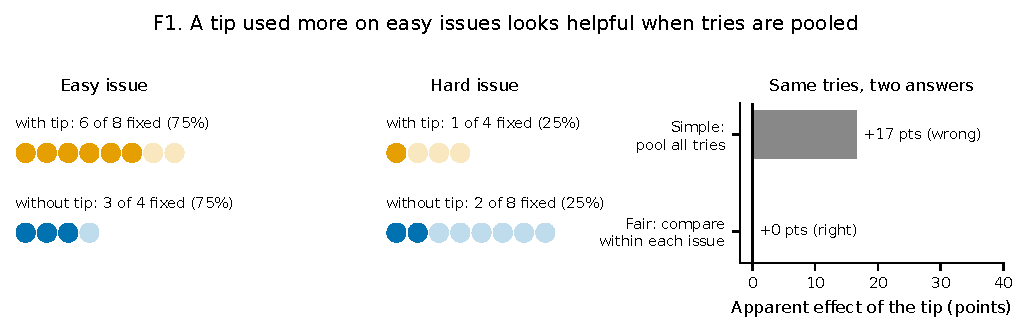
\includegraphics[width=\textwidth]{f1_method.pdf}
  \Description{Toy example with an easy and a hard issue; pooling gives +17 points, within-issue comparison gives 0.}
  \caption{Why pooled comparisons mislead. Within each issue the tip changes nothing, but it is used more on the easy issue, so pooling all attempts makes it look helpful. Our estimator compares attempts within an issue and then averages.}
  \label{fig:method}
\end{figure*}

% ---------------------------------------------------------------------------
\section{Related Work}

\paragraph{Trajectory analyses.} Many studies relate agent behavior to success: action patterns and behavioral profiles~\cite{gao2026interpret}, behavioral drivers across agents~\cite{mehtiyev2026beyond}, and the role of reproduction tests in repair~\cite{ceka2025traceability}. These are observational and compare runs across tasks. Khanna~\cite{khanna2026sametask} shows that such pooled comparisons are inflated by between-task structure and recommends within-task comparisons and permutation calibration. We adopt that recommendation, add a version control and coin-flip framing, and measure named tips across eight AI configurations.

\paragraph{Identification from sampling noise.} He et al.~\cite{he2026process} note that, given a history, the next action is randomized by decoding noise, and they estimate step effects by \emph{replaying} continuations from prefixes. We use the same logic without replay, relying on attempts that already exist in public logs; at our scale, population-level effects are well powered. Sam-Bodden~\cite{sambodden2026context} reports that even temperature-0 inference flips about 9\% of per-instance outcomes, which supports the premise that repeated attempts differ by chance.

\paragraph{Interventions on instructions.} Prompt studies find that repository context files push agents toward more exploration and testing without higher success~\cite{gloaguen2026agentsmd}, and that an instruction only to reproduce before patching does not help and can hurt~\cite{gloaguen2026act}. Our results agree, using natural variation on real issues rather than modified tasks.

% ---------------------------------------------------------------------------
\section{Data}

We use three public datasets (Table~\ref{tab:data} lists their Hugging Face IDs), each pinned to a Hugging Face revision with SHA-256 checksums.

\begin{itemize}
  \item \textbf{Older AI}~\cite{nebius2024trajectories}: SWE-agent runs of the \path{swe-agent-llama-70b} model on SWE-bench-style issues~\cite{jimenez2024swebench}, with a median of \OlderTriesPerIssue{} attempts per issue, with evaluation timestamps.
  \item \textbf{Nebius newer AI}~\cite{nebius2025openhands}: OpenHands runs of Qwen3-Coder on SWE-rebench issues~\cite{badertdinov2025swerebench}. It keeps every attempt, including failures.
  \item \textbf{NVIDIA newer AIs}~\cite{ahmad2026openswetraces}: Open-SWE-Traces. We use the \NumNewerConfigs{} subsets (\NumNewerModels{} models across SWE-agent and OpenHands, two task sources) that have repeated attempts per issue and a shared editing tool.
\end{itemize}

\paragraph{Cleaning.} We converted all \TriesTotal{} attempts and \StepsTotal{}M steps into one schema (Table~\ref{tab:funnel}). We kept attempts whose issue text matches the most common text for that issue (so inputs are identical), dropped NVIDIA attempts with unknown outcome, and, for the older AI, kept attempts restricted to the target model. NVIDIA had already removed attempts that hit the step limit or produced no patch~\cite{ahmad2026openswetraces}; Section~\ref{sec:threats} discusses this.

\paragraph{Hidden model versions.} The older dataset's single model label covers several versions: success rates by evaluation day range from \VersionRateMin{} to \VersionRateMax{}, and the share of attempts that start by writing a script moves with them (Figure~\ref{fig:versions}). We therefore compare attempts within issue \emph{and} evaluation day.

\begin{figure}[t]
  \centering
  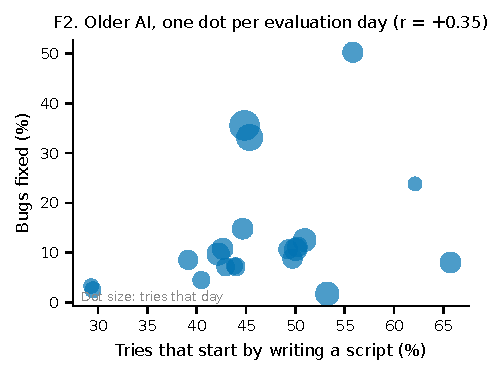
\includegraphics[width=\columnwidth]{f2_versions.pdf}
  \Description{Scatter of evaluation days: share of attempts starting with a script versus success rate.}
  \caption{Older AI by evaluation day: success and the share of attempts that start by writing a script move together, revealing a mixture of model versions.}
  \label{fig:versions}
\end{figure}

\paragraph{Labels.} A shared rule-based labeler maps every action to one of twelve kinds (e.g.\ create reproduction script, edit code, run, run test suite, look). We validated it in two ways. First, we checked each label against the tool's reply (e.g.\ a ``create'' was confirmed by the file-created message). Second, a blind second labeling of stratified samples agreed with the rules with Cohen's $\kappa$~\cite{cohen1960} of \KappaOne{} ($n=\LabelNOne$) and, on a fresh sample, \KappaTwo{} ($n=\LabelNTwo$). The reproduction-script label has precision \ReproPrecision{} and recall \ReproRecall{}; we test the effect of missed scripts in Section~\ref{sec:robust}.

\begin{table*}[t]
  \caption{Datasets as analysed (attempts with identical input and known outcome).}
  \label{tab:data}
  \footnotesize
  \resizebox{\textwidth}{!}{\begin{tabular}{llrrrrr}
\toprule
Dataset & Source (revision) & Tries & Issues & Tries per issue (median) & Steps & Bugs fixed \\
\midrule
Older AI (SWE-agent 2024, Llama-70B) & nebius/SWE-agent-trajectories (68195a1) & 73,738 & 3,591 & 13 & 1,933,044 & 16.4\% \\
Nebius OpenHands (Qwen3-Coder) & nebius/SWE-rebench-openhands-trajectories (3545538) & 67,049 & 6,306 & 10 & 4,316,962 & 48.0\% \\
NVIDIA Open-SWE-Traces (4 AIs, 7 configurations) & nvidia/Open-SWE-Traces (1db6741) & 212,222 & 99,018 & 2 & 20,230,229 & 45.2\% \\
\bottomrule
\end{tabular}
}
\end{table*}

% ---------------------------------------------------------------------------
\section{Fair-Comparison Method}

\paragraph{Estimator.} For a binary choice $a$ vs.\ $b$ (e.g.\ reproduce first vs.\ search first) we form strata: issue $\times$ day for the older AI, and AI configuration $\times$ issue for the newer AIs. In stratum $s$ with $n_{as}$ and $n_{bs}$ attempts and success rates $\hat p_{as}$, $\hat p_{bs}$, the estimate is the Mantel--Haenszel-weighted~\cite{mantel1959} average of within-stratum differences,
\[
  \hat\Delta = \frac{\sum_s w_s(\hat p_{as}-\hat p_{bs})}{\sum_s w_s},\qquad w_s=\frac{n_{as}n_{bs}}{n_{as}+n_{bs}},
\]
using only strata that contain both groups. We report 95\% (and 90\%) CIs from 2,000 bootstrap resamples of whole issues, and a permutation $p$-value from 1,000 shuffles of group labels within strata. As cross-checks we fit a linear probability model with stratum fixed effects and issue-clustered standard errors~\cite{cameron2015,angrist2009}, and a conditional logistic regression. The \emph{simple} estimate is the pooled difference in success rates with no strata.

\paragraph{Hypotheses.} \textbf{P1}: for the older AI, the first action is \texttt{create} (group R) vs.\ a search or navigation command (group S). \textbf{P2}: for the newer AIs, the attempt creates a test or reproduction file before its first edit of project code (``test first'') vs.\ edits code first (``fix first''). ``No meaningful difference'' is claimed only if the 90\% CI lies within $\pm$\Margin{} points (two one-sided tests~\cite{schuirmann1987}). \textbf{P3}: the mean absolute gap between simple and fair estimates, over all tip--AI pairs, exceeds 2 points. Thirteen secondary analyses (\NumSecondary{} estimates) are corrected together with Benjamini--Hochberg~\cite{benjamini1995} at $q=0.05$. Comparisons with fewer than 100 informative strata are labelled underpowered and not interpreted.

\paragraph{What is and is not a coin flip.} P1 is a decision at the first step, made on identical input, so within an issue and day it is as good as random (we test this below). P2 and the after-fix tips (S1--S6) are decisions made mid-run, after the agent has seen some output. For these, within-issue comparisons remove issue difficulty but not everything the agent observed, so we call them same-issue associations. For P2 we add a stricter check: pairs of attempts with \emph{identical} action histories up to the point where one creates a test file and the other does something else.

\paragraph{Design checks.} (i) Within issue $\times$ day, the evaluation hour does not predict the first move (permutation $p=\HourBalanceP$, \HourBalanceGroups{} groups). (ii) A placebo comparing two names for the same action, \texttt{reproduce.py} vs.\ \texttt{reproduce\_bug.py}, gives \Placebo{} points (95\% CI \PlaceboLo{} to \PlaceboHi{}). (iii) We verify that each AI is ``undecided'' about the tip, choosing it in between 5\% and 95\% of attempts; test-first rates in the NVIDIA configurations range from \ComplianceMin{} to \ComplianceMax{}, while the Nebius Qwen3-Coder tests first in \NebiusCompliance{} of attempts and therefore offers no natural experiment for P2.

% ---------------------------------------------------------------------------
\section{Results}

Table~\ref{tab:primary} summarises the primary results.

\begin{table*}[t]
  \caption{Primary estimates, in bugs fixed per 100 attempts (95\% CI). Groups / issues / attempts refer to the fair comparison.}
  \label{tab:primary}
  \footnotesize
  \resizebox{\textwidth}{!}{\begin{tabular}{lllllll}
\toprule
Hypothesis & Fair (95\% CI) & Permutation p & FE regression & Simple & Groups / issues / tries & Decision \\
\midrule
P1 Reproduce first (older AI) & -3.5 [-4.8, -2.2] & <0.001 & -3.5 [-4.9, -2.1] & -2.8 [-5.2, -0.4] & 1,870 / 1,048 / 13,509 & harm \\
P2 Test first (newer AIs, pooled) & +0.1 [-0.5, +0.6] & 0.803 & +0.1 [-0.6, +0.8] & +1.9 [+1.2, +2.5] & 9,776 / 9,776 / 25,773 & equivalent within $\pm$2 points \\
P3 Mean |simple $-$ fair| over tip $\times$ AI pairs & 10.9 [10.3, 11.9] & — & — & — & 57 pairs & supported (> 2 pts) \\
\bottomrule
\end{tabular}
}
\end{table*}

\subsection{Reproducing first hurt the older AI (P1)}

Within issue and day, attempts that began by creating a script resolved \POneAbs{} fewer issues per 100 (95\% CI \POneLo{} to \POneHi{}; permutation $p\,\POneP$; \POneGroups{} groups, \POneIssues{} issues, \POneTries{} attempts). The fixed-effects regression gives \POneFE{} points and the conditional logit an odds ratio of \ORPOne{}. The effect is stable across five definitions of the version batch (\BatchMin{} to \BatchMax{}; Figure~\ref{fig:older}).

\begin{figure}[t]
  \centering
  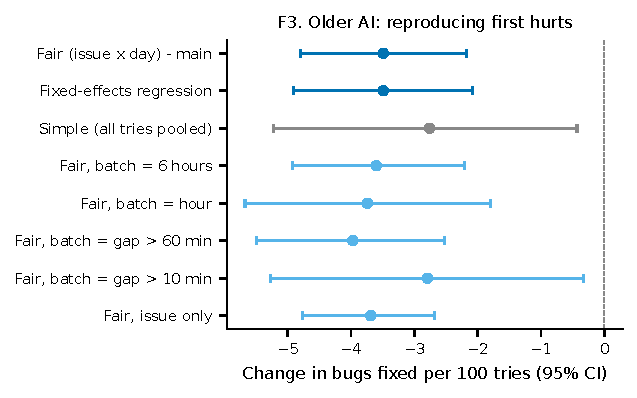
\includegraphics[width=\columnwidth]{f3_older.pdf}
  \Description{Forest plot: all estimates of the reproduce-first effect for the older AI are between about -2.8 and -4 points with confidence intervals below zero.}
  \caption{P1 under the main design, the alternative estimators, and alternative version-batch definitions. All 95\% CIs exclude zero.}
  \label{fig:older}
\end{figure}

\subsection{Why: context and localization}

Reproducing first was costly. Within the same issue and day, it added \CostStepsOlder{} steps per attempt and raised the share of attempts that ran out of context by \CtxExit{} points (Figure~\ref{fig:mechanism}a). It also delayed localization: the median step at which the agent first opened a file changed by the reference fix was \KMMedianR{} for reproduce-first attempts and \KMMedianS{} for search-first attempts (Kaplan--Meier~\cite{kaplan1958}; Figure~\ref{fig:mechanism}b). A discrete-time hazard model puts the per-step chance of reaching the gold file \Hazard{} points lower. An agent with a small context window pays for the script with the room it needs to find and fix the bug.

\begin{figure*}[t]
  \centering
  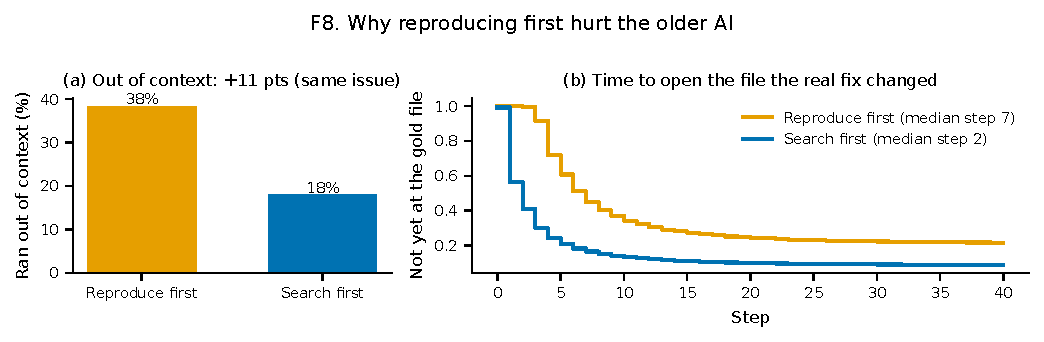
\includegraphics[width=\textwidth]{f8_mechanism.pdf}
  \Description{Left: bar chart of context exhaustion, higher for reproduce first. Right: survival curves showing reproduce-first attempts reach the gold file later.}
  \caption{Mechanism for the older AI. (a) Share of attempts that ran out of context. (b) Time to first open a file changed by the reference fix; attempts that never open one are censored.}
  \label{fig:mechanism}
\end{figure*}

\subsection{Testing first made no difference for newer AIs (P2)}

Pooled over the \NumNewerConfigs{} newer configurations, testing first changed success by \PTwoEst{} points (95\% CI \PTwoLo{} to \PTwoHi{}; 90\% CI \PTwoLoNinety{} to \PTwoHiNinety{}; \PTwoIssues{} issues), which is equivalent to zero within $\pm$\Margin{} points. Per-configuration estimates range from \PerAIFairMin{} to \PerAIFairMax{} (Figure~\ref{fig:newer}). We found \ForkPairs{} pairs of attempts with identical action histories; in the \ForkN{} attempts where, at the fork, one creates a test file and the other does something else, creating the test file changed success by \ForkEst{} points (95\% CI \ForkLo{} to \ForkHi{}). The conditional logit odds ratio is \ORPTwo{}. For the Nebius Qwen3-Coder, which almost always tests first, the one available coin flip at the first step (\texttt{think} vs.\ \texttt{view}) also shows no effect (\STwelve{} points; 95\% CI \STwelveLo{} to \STwelveHi{}).

Testing first is not free for newer AIs either: it costs \CostStepsNewer{} more steps, \CostReadNewer{}k more characters read and \CostWriteNewer{}k more written per attempt (Figure~\ref{fig:cost}). A plausible but untested explanation for the different outcome is that newer models have larger context windows, so the extra cost does not turn into failures.

\begin{figure}[t]
  \centering
  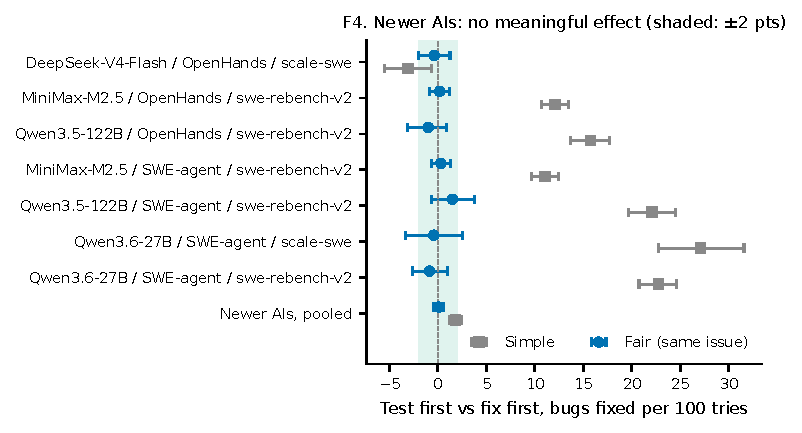
\includegraphics[width=\columnwidth]{f4_newer.pdf}
  \Description{Forest plot per AI: simple estimates range up to +27 points while fair estimates stay within about one point of zero.}
  \caption{P2 per AI configuration and pooled. Simple pooled estimates (grey) suggest large benefits; within-issue estimates (blue) are all close to zero. Shaded: the pre-registered $\pm$\Margin{}-point equivalence margin.}
  \label{fig:newer}
\end{figure}

\begin{figure}[t]
  \centering
  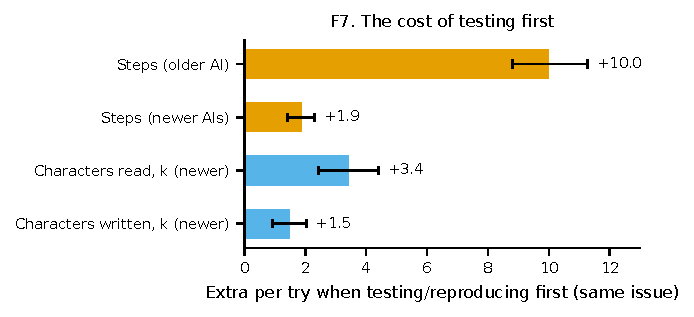
\includegraphics[width=\columnwidth]{f7_cost.pdf}
  \Description{Bar chart of extra steps and characters per attempt when testing first.}
  \caption{Extra cost per attempt of testing or reproducing first, within the same issue.}
  \label{fig:cost}
\end{figure}

\subsection{Simple analyses mislead (P3)}

For every tip--AI pair we computed both the simple pooled difference and the fair within-issue difference (Figure~\ref{fig:gaps}). The mean absolute gap is \PThreeGap{} points (95\% CI \PThreeLo{} to \PThreeHi{}) over \PThreePairs{} pairs; the two point in opposite directions in \PThreeSign{} of pairs and disagree on statistical significance in \PThreeSig{}. Leaving out the underpowered pairs gives \PThreeExGap{} points over \PThreeExPairs{} pairs. The P2 data also show Simpson's paradox: pooled across AIs, the simple estimate is \PTwoSimple{} points, while the per-AI simple estimates range from \PerAISimpleMin{} to \PerAISimpleMax{}, and the fair estimates from \PerAIFairMin{} to \PerAIFairMax{}. A study that compared successful and failed runs on this data would conclude that testing first adds up to \PerAISimpleMax{} points for some AIs; within the same issue, it adds nothing measurable.

\begin{figure}[t]
  \centering
  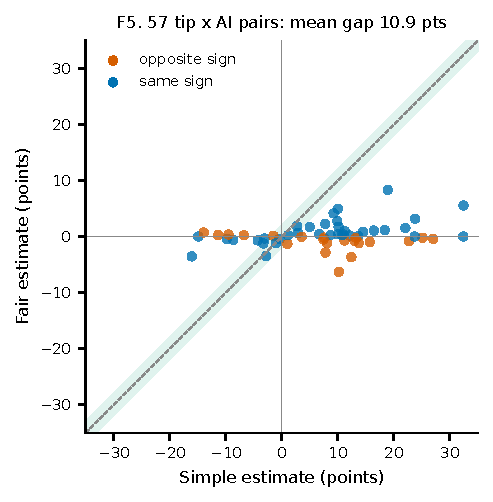
\includegraphics[width=\columnwidth]{f5_gaps.pdf}
  \Description{Scatter of simple versus fair estimates; most points lie far from the diagonal, many with opposite signs.}
  \caption{Simple vs.\ fair estimates for every tip--AI pair. Points far from the diagonal are pairs where a pooled analysis misleads; red points flip sign. Shaded band: within 2 points.}
  \label{fig:gaps}
\end{figure}

\subsection{Other tips}

Of \NumSecondary{} secondary estimates, \NumSecondarySig{} remain significant after correction (Figure~\ref{fig:tips}; full list in Table~\ref{tab:secondary}). Re-running one's own test or reproduction script after the first fix (``check your fix'') is associated with \SOneOlder{} points for the older AI (95\% CI \SOneOlderLo{} to \SOneOlderHi{}) and \SOneTopNewer{} points for \SOneTopNewerAI{}; its CI includes zero for the other six configurations. Running the project's test suite, writing extra tests, and cleaning up show no consistent association. For the older AI, the choice among search commands as a first move makes little difference (\SThirteenMin{} to \SThirteenMax{} points vs.\ \texttt{search\_dir}). No interaction with issue type or programming language survived correction.

\begin{figure*}[t]
  \centering
  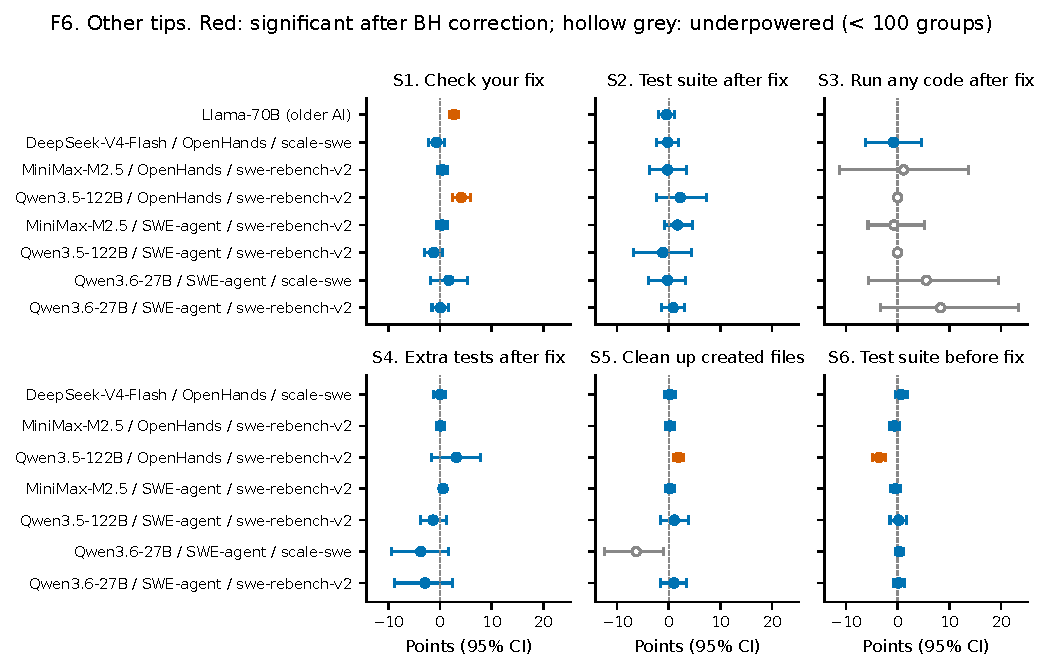
\includegraphics[width=\textwidth]{f6_tips.pdf}
  \Description{Six forest plots of other tips per AI; most intervals include zero.}
  \caption{Other tips, fair within-issue estimates per AI configuration. These are same-issue associations, not coin flips.}
  \label{fig:tips}
\end{figure*}

% ---------------------------------------------------------------------------
\section{Robustness}
\label{sec:robust}

\paragraph{Version batches and undated attempts.} Some older-AI attempts lack an evaluation time; all of them failed. Adding them back to their issue in proportion to other failures gives \UndatedImputed{} points; the most adverse possible placement, one attempt at a time, gives \UndatedWorst{} points.

\paragraph{Leave one AI out.} Dropping any one newer configuration keeps every 90\% CI for P2 within \LOOLo{} to \LOOHi{} points.

\paragraph{Label errors.} A missed reproduction script can only move an attempt from ``fix first'' to ``test first'' if the attempt created some file before its first fix. Moving all such attempts gives \Broad{} points (95\% CI \BroadLo{} to \BroadHi{}).

\paragraph{Reproducibility.} Running the full analysis twice from scratch yields \Reproducible{} result tables.

% ---------------------------------------------------------------------------
\section{Threats to Validity}
\label{sec:threats}

\paragraph{NVIDIA's filtering.} NVIDIA removed attempts that hit the step limit or produced no patch. These are hidden failures. If test-first attempts lost \TipPoint{} more of them than fix-first attempts, P2 would reach $-$\Margin{} points. We calibrated this with the unfiltered Nebius data: there, the share of attempts that such filtering would remove is \Calib{} points lower for test-first than fix-first attempts (95\% CI \CalibLo{} to \CalibHi{}; \CalibIssues{} issues), so the filter, if anything, works against testing first. The calibration comes from a different AI and few issues, so this remains the main limitation of P2.

\paragraph{Mid-run decisions.} P2 and S1--S6 are not decided at the first step. Within-issue comparisons remove issue difficulty but not what the agent saw before deciding. The exact-fork analysis addresses this for P2; for S1--S6 we make no causal claim.

\paragraph{Version proxy.} The evaluation day is a proxy for the older model's version. Finer batches (hours, bursts separated by 10- or 60-minute gaps) give the same answer.

\paragraph{Labels and AI-assisted validation.} The second labeling used in the label validation was performed with the help of an AI assistant rather than a human annotator, blind to the rule labels. We disclose this and publish both labelings; the primary evidence for label quality is the check against tool replies, which is independent of any annotator.

\paragraph{Generalization.} The older AI is a 2024 open model; the newer AIs are recent open models. Results may differ for proprietary agents, other scaffolds, or tasks without hidden tests.

% ---------------------------------------------------------------------------
\section{Discussion}

For an older, context-limited agent, reproducing the bug first was harmful: the script used up space and time the agent needed to find the bug. For newer agents, testing first neither helped nor hurt, at a measurable cost in steps and text. ``Check your fix'' is the only tip with a positive association, and only for some AIs. A practical reading is that process advice should be evaluated per agent, and that its cost matters when context is scarce.

The larger lesson is methodological. Pooled comparisons of successful and failed runs, the most common analysis of agent trajectories, were off by \PThreeGap{} points on average in our data, often in the wrong direction. Repeated attempts of the same issue are already common in public datasets; comparing within them is cheap and much more reliable.

\section{Conclusion}

Using natural experiments in repeated agent attempts, we found that the popular advice to reproduce a bug first hurt an older coding agent and made no difference for \NumNewerModels{} newer ones, while simple analyses of the same data suggest large benefits. We recommend within-issue comparisons as the default for analysing agent trajectories.

\section{Data and Code Availability}

All datasets are public on Hugging Face; the exact revisions and checksums are listed in the repository. The code (MIT license), including the cleaning, labeling, estimation, robustness, figure and table steps, is available at \url{https://github.com/rajanyadav0307/tips_agentic_ai}. The command \texttt{agent-tips run-all} reproduces every number, figure and table in this paper from the raw data. The analysis plan was frozen in the repository (tag \texttt{analysis-plan-v1}) before the confirmatory runs.

\paragraph{Use of generative AI.} AI coding and writing assistants were used to implement the pipeline, perform the second labeling for label validation (Section~\ref{sec:threats}), and draft this manuscript. The author reviewed all code, results and text and takes responsibility for them.

\bibliographystyle{ACM-Reference-Format}
\bibliography{refs}

\appendix
\section{Cleaning funnel}

\begin{table*}[h]
  \caption{Cleaning funnel per dataset.}
  \label{tab:funnel}
  \footnotesize
  \begin{tabular}{llrrrr}
\toprule
Dataset & Stage & Tries & Issues & Removed & Bugs fixed \\
\midrule
Older AI & All tries in the dataset & 80,036 & 3,591 & — & 16.7\% \\
Older AI & In scope (swe-agent-llama-70b) & 74,792 & 3,591 & 5,244 & 16.7\% \\
Older AI & Same issue text as the most common one & 73,738 & 3,591 & 1,054 & 16.4\% \\
Older AI & Dated (evaluation timestamp found) & 63,269 & 3,490 & 10,469 & 19.1\% \\
Nebius OpenHands & All tries in the dataset & 67,074 & 6,306 & — & 47.9\% \\
Nebius OpenHands & Same issue text as the most common one & 67,049 & 6,306 & 25 & 47.9\% \\
NVIDIA Open-SWE-Traces & All tries in the 7 subsets & 254,933 & 117,664 & — & 45.2\% \\
NVIDIA Open-SWE-Traces & Outcome known (resolved is 0 or 1) & 212,222 & 99,018 & 42,711 & 45.2\% \\
NVIDIA Open-SWE-Traces & Same issue text as the most common one & 212,222 & 99,018 & 0 & 45.2\% \\
\bottomrule
\end{tabular}

\end{table*}

\section{All secondary estimates}

\begin{table*}[h]
  \caption{All secondary estimates (fair, within-issue), with Benjamini--Hochberg $q$-values. Points per 100 attempts unless the outcome is a count.}
  \label{tab:secondary}
  \scriptsize
  \resizebox{\textwidth}{!}{\begin{tabular}{llllrrl}
\toprule
ID & Question & AI & Estimate (95\% CI) & Groups & q & Sig. \\
\midrule
S1 & Check your fix & Llama-70B (older AI) & +2.7 [+1.9, +3.6] pts & 4,669 & 0.007 & yes \\
S1 & Check your fix & DeepSeek-V4-Flash / OpenHands / scale-swe & -0.7 [-2.2, +0.8] pts & 1,011 & 0.797 &  \\
S1 & Check your fix & MiniMax-M2.5 / OpenHands / swe-rebench-v2 & +0.4 [-0.5, +1.4] pts & 2,710 & 0.797 &  \\
S1 & Check your fix & Qwen3.5-122B / OpenHands / swe-rebench-v2 & +4.1 [+2.4, +5.9] pts & 1,508 & 0.007 & yes \\
S1 & Check your fix & MiniMax-M2.5 / SWE-agent / swe-rebench-v2 & +0.4 [-0.6, +1.4] pts & 3,264 & 0.797 &  \\
S1 & Check your fix & Qwen3.5-122B / SWE-agent / swe-rebench-v2 & -1.2 [-3.0, +0.6] pts & 1,145 & 0.695 &  \\
S1 & Check your fix & Qwen3.6-27B / SWE-agent / scale-swe & +1.7 [-1.8, +5.3] pts & 231 & 0.797 &  \\
S1 & Check your fix & Qwen3.6-27B / SWE-agent / swe-rebench-v2 & +0.1 [-1.5, +1.7] pts & 1,503 & 1.000 &  \\
S2 & Test suite after fix & Llama-70B (older AI) & -0.4 [-2.1, +1.1] pts & 1,388 & 0.847 &  \\
S2 & Test suite after fix & DeepSeek-V4-Flash / OpenHands / scale-swe & -0.2 [-2.4, +2.0] pts & 507 & 1.000 &  \\
S2 & Test suite after fix & MiniMax-M2.5 / OpenHands / swe-rebench-v2 & -0.2 [-3.8, +3.4] pts & 230 & 1.000 &  \\
S2 & Test suite after fix & Qwen3.5-122B / OpenHands / swe-rebench-v2 & +2.2 [-2.4, +7.3] pts & 174 & 0.797 &  \\
S2 & Test suite after fix & MiniMax-M2.5 / SWE-agent / swe-rebench-v2 & +1.7 [-0.9, +4.6] pts & 474 & 0.695 &  \\
S2 & Test suite after fix & Qwen3.5-122B / SWE-agent / swe-rebench-v2 & -1.2 [-6.8, +4.3] pts & 171 & 0.977 &  \\
S2 & Test suite after fix & Qwen3.6-27B / SWE-agent / scale-swe & -0.2 [-3.9, +3.3] pts & 235 & 1.000 &  \\
S2 & Test suite after fix & Qwen3.6-27B / SWE-agent / swe-rebench-v2 & +0.8 [-1.4, +3.1] pts & 631 & 0.797 &  \\
S3 & Run any code after fix & DeepSeek-V4-Flash / OpenHands / scale-swe & -0.8 [-6.2, +4.7] pts & 129 & 1.000 &  \\
S3 & Run any code after fix & MiniMax-M2.5 / OpenHands / swe-rebench-v2 & +1.1 [-11.2, +13.8] pts & 24 & 1.000 & underpowered \\
S3 & Run any code after fix & Qwen3.5-122B / OpenHands / swe-rebench-v2 & +0.0 [+0.0, +0.0] pts & 8 & 1.000 & underpowered \\
S3 & Run any code after fix & MiniMax-M2.5 / SWE-agent / swe-rebench-v2 & -0.7 [-5.7, +5.2] pts & 38 & 1.000 & underpowered \\
S3 & Run any code after fix & Qwen3.5-122B / SWE-agent / swe-rebench-v2 & +0.0 [+0.0, +0.0] pts & 12 & 1.000 & underpowered \\
S3 & Run any code after fix & Qwen3.6-27B / SWE-agent / scale-swe & +5.6 [-5.6, +19.4] pts & 19 & 0.847 & underpowered \\
S3 & Run any code after fix & Qwen3.6-27B / SWE-agent / swe-rebench-v2 & +8.3 [-3.4, +23.4] pts & 27 & 0.745 & underpowered \\
S4 & Extra tests after fix & DeepSeek-V4-Flash / OpenHands / scale-swe & +0.0 [-1.2, +1.1] pts & 2,279 & 1.000 &  \\
S4 & Extra tests after fix & MiniMax-M2.5 / OpenHands / swe-rebench-v2 & +0.1 [-0.7, +0.9] pts & 4,999 & 1.000 &  \\
S4 & Extra tests after fix & Qwen3.5-122B / OpenHands / swe-rebench-v2 & +3.2 [-1.6, +7.8] pts & 156 & 0.695 &  \\
S4 & Extra tests after fix & MiniMax-M2.5 / SWE-agent / swe-rebench-v2 & +0.6 [-0.2, +1.4] pts & 5,514 & 0.593 &  \\
S4 & Extra tests after fix & Qwen3.5-122B / SWE-agent / swe-rebench-v2 & -1.3 [-3.7, +1.2] pts & 572 & 0.797 &  \\
S4 & Extra tests after fix & Qwen3.6-27B / SWE-agent / scale-swe & -3.7 [-9.4, +1.6] pts & 105 & 0.695 &  \\
S4 & Extra tests after fix & Qwen3.6-27B / SWE-agent / swe-rebench-v2 & -2.9 [-8.8, +2.4] pts & 130 & 0.797 &  \\
S5 & Clean up created files & DeepSeek-V4-Flash / OpenHands / scale-swe & +0.3 [-0.7, +1.3] pts & 2,324 & 0.940 &  \\
S5 & Clean up created files & MiniMax-M2.5 / OpenHands / swe-rebench-v2 & +0.2 [-0.7, +1.2] pts & 3,281 & 0.856 &  \\
S5 & Clean up created files & Qwen3.5-122B / OpenHands / swe-rebench-v2 & +1.8 [+0.9, +2.8] pts & 4,032 & 0.007 & yes \\
S5 & Clean up created files & MiniMax-M2.5 / SWE-agent / swe-rebench-v2 & +0.2 [-0.6, +1.1] pts & 3,899 & 0.912 &  \\
S5 & Clean up created files & Qwen3.5-122B / SWE-agent / swe-rebench-v2 & +1.1 [-1.6, +3.9] pts & 634 & 0.797 &  \\
S5 & Clean up created files & Qwen3.6-27B / SWE-agent / scale-swe & -6.3 [-12.4, -0.9] pts & 85 & 0.122 & underpowered \\
S5 & Clean up created files & Qwen3.6-27B / SWE-agent / swe-rebench-v2 & +1.0 [-1.5, +3.5] pts & 322 & 0.801 &  \\
S6 & Test suite before fix & DeepSeek-V4-Flash / OpenHands / scale-swe & +0.7 [-0.4, +1.9] pts & 1,854 & 0.797 &  \\
S6 & Test suite before fix & MiniMax-M2.5 / OpenHands / swe-rebench-v2 & -0.6 [-1.6, +0.3] pts & 3,353 & 0.720 &  \\
S6 & Test suite before fix & Qwen3.5-122B / OpenHands / swe-rebench-v2 & -3.6 [-4.8, -2.3] pts & 2,807 & 0.007 & yes \\
S6 & Test suite before fix & MiniMax-M2.5 / SWE-agent / swe-rebench-v2 & -0.4 [-1.4, +0.6] pts & 3,440 & 0.797 &  \\
S6 & Test suite before fix & Qwen3.5-122B / SWE-agent / swe-rebench-v2 & +0.2 [-1.5, +1.8] pts & 1,486 & 1.000 &  \\
S6 & Test suite before fix & Qwen3.6-27B / SWE-agent / scale-swe & +0.4 [-0.4, +1.1] pts & 3,367 & 0.797 &  \\
S6 & Test suite before fix & Qwen3.6-27B / SWE-agent / swe-rebench-v2 & +0.2 [-0.8, +1.3] pts & 2,888 & 1.000 &  \\
S7 & Cost: steps & Llama-70B (older AI) & +10.0 [+8.8, +11.3] & 1,870 & 0.007 & yes \\
S7 & Cost: steps & Newer AIs, pooled & +1.9 [+1.4, +2.3] & 9,776 & 0.007 & yes \\
S7 & Cost: characters read (thousands) & Newer AIs, pooled & +3.4 [+2.4, +4.4] & 9,776 & 0.007 & yes \\
S7 & Cost: characters written (thousands) & Newer AIs, pooled & +1.5 [+0.9, +2.0] & 9,776 & 0.007 & yes \\
S9 & Test first, language = go & Newer AIs, pooled & +0.1 [-1.3, +1.6] pts & 1,730 & 1.000 &  \\
S9 & Test first, language = java & Newer AIs, pooled & +1.5 [-1.4, +4.5] pts & 403 & 0.797 &  \\
S9 & Test first, language = javascript & Newer AIs, pooled & +0.5 [-1.0, +2.1] pts & 1,171 & 0.801 &  \\
S9 & Test first, language = php & Newer AIs, pooled & +2.5 [-0.8, +5.6] pts & 347 & 0.593 &  \\
S9 & Test first, language = python & Newer AIs, pooled & -0.1 [-0.9, +0.7] pts & 3,851 & 1.000 &  \\
S9 & Test first, language = rust & Newer AIs, pooled & -1.1 [-3.1, +0.8] pts & 750 & 0.797 &  \\
S9 & Test first, language = typescript & Newer AIs, pooled & -0.1 [-1.6, +1.6] pts & 1,486 & 1.000 &  \\
S10 & Submitted because the context ran out & Llama-70B (older AI) & +11.0 [+9.2, +12.8] pts & 1,870 & 0.007 & yes \\
S10 & Any context-limit exit & Llama-70B (older AI) & +11.0 [+9.1, +12.8] pts & 1,870 & 0.007 & yes \\
S12 & First move think vs view (Qwen3-Coder) & Qwen3-Coder & -0.1 [-0.7, +0.6] pts & 2,067 & 1.000 &  \\
S13 & First move find\_file vs search\_dir & Llama-70B (older AI) & -0.5 [-2.0, +1.0] pts & 1,485 & 0.801 &  \\
S13 & First move ls vs search\_dir & Llama-70B (older AI) & -1.2 [-2.5, +0.1] pts & 1,697 & 0.354 &  \\
S13 & First move open vs search\_dir & Llama-70B (older AI) & +5.0 [-1.1, +11.3] pts & 136 & 0.593 &  \\
S13 & First move grep vs search\_dir & Llama-70B (older AI) & -1.2 [-4.0, +1.4] pts & 395 & 0.797 &  \\
S8 & Reproduce first x issue type: has\_code\_block & Llama-70B (older AI) & +2.6 [-1.0, +6.2] pts & — & 0.680 &  \\
S8 & Reproduce first x issue type: has\_stack\_trace & Llama-70B (older AI) & -1.9 [-6.3, +2.5] pts & — & 0.797 &  \\
S8 & Reproduce first x issue type: names\_file & Llama-70B (older AI) & -0.8 [-4.5, +2.9] pts & — & 0.953 &  \\
S8 & Reproduce first x issue type: long\_issue & Llama-70B (older AI) & +0.2 [-3.8, +4.1] pts & — & 1.000 &  \\
S9 & Test first x language (vs python): lang\_go & Newer AIs, pooled & +0.2 [-1.9, +2.3] pts & — & 1.000 &  \\
S9 & Test first x language (vs python): lang\_java & Newer AIs, pooled & +1.6 [-2.3, +5.5] pts & — & 0.797 &  \\
S9 & Test first x language (vs python): lang\_javascript & Newer AIs, pooled & +0.7 [-1.5, +2.9] pts & — & 0.847 &  \\
S9 & Test first x language (vs python): lang\_php & Newer AIs, pooled & +2.6 [-1.6, +6.8] pts & — & 0.731 &  \\
S9 & Test first x language (vs python): lang\_rust & Newer AIs, pooled & -1.0 [-3.8, +1.8] pts & — & 0.801 &  \\
S9 & Test first x language (vs python): lang\_typescript & Newer AIs, pooled & +0.0 [-2.2, +2.3] pts & — & 1.000 &  \\
S11 & Finding the right file: per-step hazard & Llama-70B (older AI) & -12.2 [-13.8, -10.7] pts & — & <0.001 & yes \\
\bottomrule
\end{tabular}
}
\end{table*}


\end{document}
